\documentclass[12pt, a4paper, oneside]{ctexart}
\usepackage{amsmath, amsthm, amssymb, graphicx}
\usepackage[bookmarks=true, colorlinks, citecolor=blue, linkcolor=black]{hyperref}
\usepackage{listings}
\usepackage{xcolor}
\usepackage{inconsolata}
\usepackage{booktabs}

% 定义可能使用到的颜色
\definecolor{CPPLight}  {HTML} {686868}
\definecolor{CPPSteel}  {HTML} {888888}
\definecolor{CPPDark}   {HTML} {262626}
\definecolor{CPPBlue}   {HTML} {4172A3}
\definecolor{CPPGreen}  {HTML} {487818}
\definecolor{CPPBrown}  {HTML} {A07040}
\definecolor{CPPRed}    {HTML} {AD4D3A}
\definecolor{CPPViolet} {HTML} {7040A0}
\definecolor{CPPGray}  {HTML} {B8B8B8}
\lstset{basicstyle=\ttfamily,breaklines=true}
\lstset{
    columns=fixed,       
    numbers=left,                                        % 在左侧显示行号
    numbersep=5pt,
    frame=none,                                          % 不显示背景边框
    backgroundcolor=\color[RGB]{245,245,244},            % 设定背景颜色
    keywordstyle=\color[RGB]{40,40,255},                 % 设定关键字颜色
    numberstyle=\footnotesize\color{red},           % 设定行号格式
    commentstyle=\it\color[RGB]{0,96,96},                % 设置代码注释的格式
    stringstyle=\rmfamily\slshape\color[RGB]{128,0,0},   % 设置字符串格式
    showstringspaces=false,                              % 不显示字符串中的空格
    language=c,                                        % 设置语言
    xleftmargin=1em, %整体距左侧边线的距离为2em
    morekeywords={alignas,continute,friend,register,true,alignof,decltype,goto,
    reinterpret_cast,try,asm,defult,if,return,typedef,auto,delete,inline,short,
    typeid,bool,do,int,signed,typename,break,double,long,sizeof,union,case,
    dynamic_cast,mutable,static,unsigned,catch,else,namespace,static_assert,using,
    char,enum,new,static_cast,virtual,char16_t,char32_t,explict,noexcept,struct,
    void,export,nullptr,switch,volatile,class,extern,operator,template,wchar_t,
    const,false,private,this,while,constexpr,float,protected,thread_local,
    const_cast,for,public,throw,std},
}
% 导言区

\title{计算机系统基础 \\ Lab2 Bomb Lab} % 标题
\author{姓名:傅文杰\\学号:22300240028} % 作者
\date{\today} % 日期

\begin{document}

\maketitle % 生成标题

\tableofcontents % 生成目录

\section{实验准备} % 一级标题
\subsection{获取Bomb}
\begin{itemize}
    \item 通过\href{http://autolab.sur.moe:5550/22300240028}{http://autolab.sur.moe:5550/22300240028}获取Bomb:22300240028.out,它是二进制格式的代码,无法直接查看
    \item 将其与bomb.c放入一个文件夹中便于查看 \\
    \item 在linux终端中执行./22300240028.out会看到以下文字,如果输入的答案不对,则Bomb会爆炸:\\
    \begin{figure}[htbp]
        % \centering
        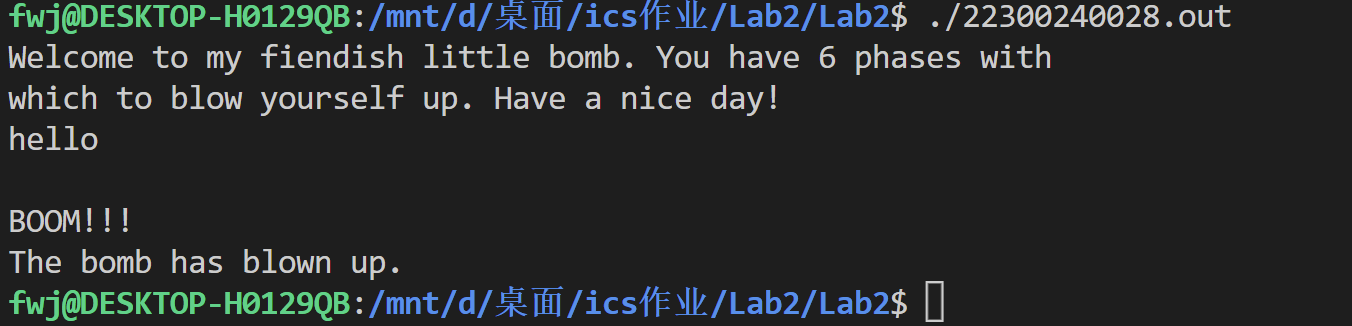
\includegraphics[scale=0.9]{image/1.1-1.png}
    \end{figure}    
\end{itemize}

\subsection{实验目的}
\begin{itemize}
    \item 这个Bomb一共有6个phase和1个secret phase需要defuse
    \item 需要将答案字符串写在.txt文件中并在最后一行写上学号
    \item 因此,我们在终端vim ans.txt创建答案文件并写入,通过./22300240028.out ans.txt并观察文字提示来判断是否成功defuse Bomb
\end{itemize}

\subsection{实验工具}
\begin{itemize}
    \item gdb\\
具体方法可以参照\href{https://linuxtools-rst.readthedocs.io/zh_CN/latest/tool/gdb.html}{gdb调试利器}或者在终端中执行man gdb,gdb -help等命令查看
    \item objdump\\
    在终端中执行:objdump 22300240028.out $>$ bomb.s 通过管道将反汇编文件保存到bomb.s中\\
    在终端中执行:objdump 22300240028.out $>$ bomb.t 可以得到符号表,可能会有些帮助 
\end{itemize}

\section{实验过程}
\subsection{观察反汇编文件bomb.s以及c语言文件bomb.c}
\begin{itemize}
    \item 观察bomb.c文件,我们可以发现其main函数通过read\_line函数读取输入,通过phase\_i$(1\le i\le 6)$函数判断是否会使炸弹爆炸
    \item 观察bomb.s文件,我们可以发现read\_line函数读入的值将会被存放在寄存器\%rdi中,再调用相对应的函数。这是因为\%rax通常作为存储函数返回值的寄存器,\%rdi通常作为存储函数第一个入参的寄存器。
          phase\_i函数使用\%rdi寄存器作为输入。
    \begin{figure}[htbp]
        % \centering
        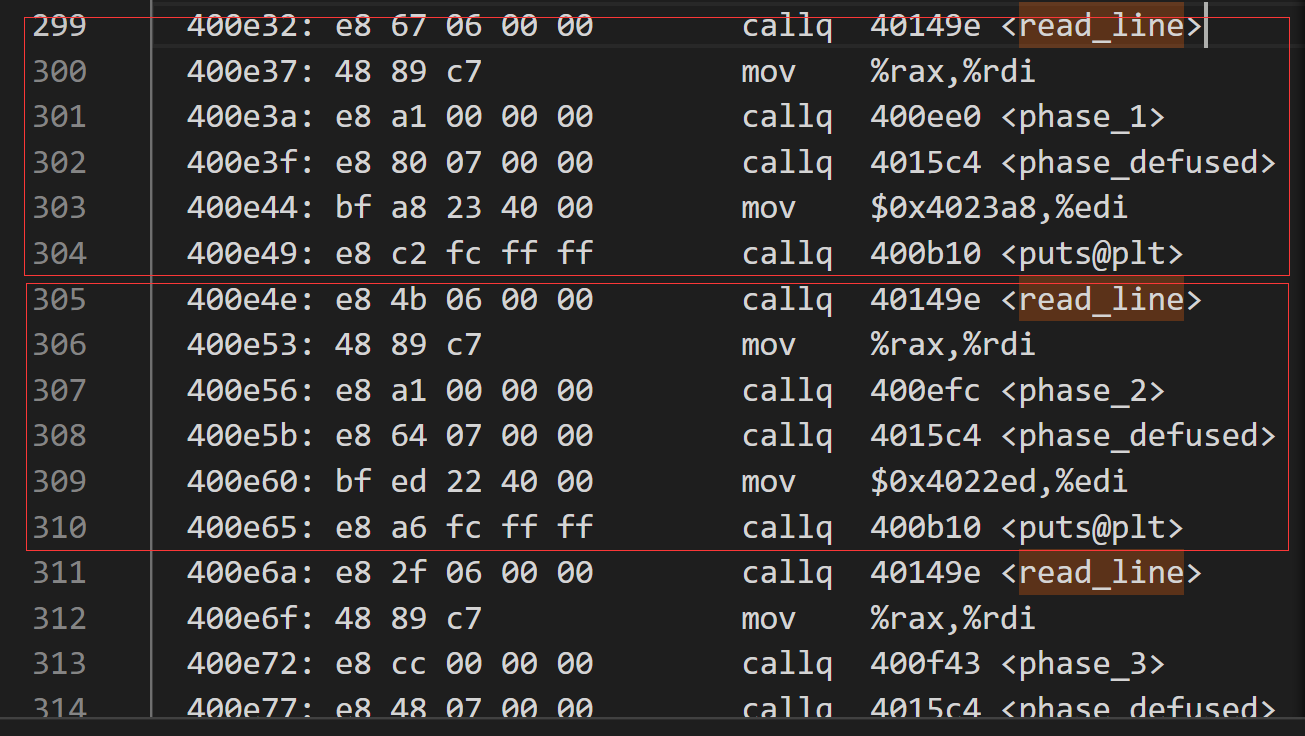
\includegraphics[scale=0.4]{image/2.1-1.png}
    \end{figure}  
    \item 我们可以在bomb.s汇编代码中通过Ctrl$+$F搜索phase\_i来观察相应的函数
\end{itemize}
\subsection{phase\_1}
\begin{figure}[htbp]
    % \centering
    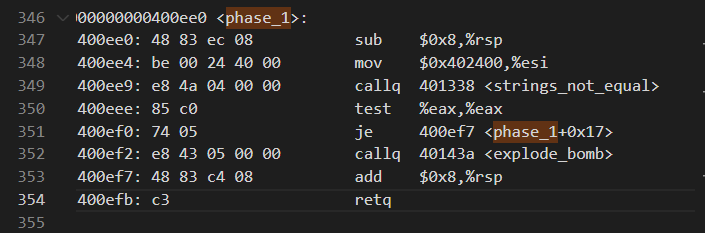
\includegraphics[scale=0.8]{image/2.2-1.png}
\end{figure} 
\begin{itemize}
    \item 第347行表示将栈顶指针$-$=8,为函数分配栈帧
    \item 第348行表示将寄存器\%rsi的后32位,即寄存器\%esi赋成立即数0x402400
    \item 第349行调用名为strings\_not\_equal的函数,猜想寄存器\%esi应该存储了该函数的入参,该函数可能是判断字符串是否相等的函数
    \item 第350行用test指令检查寄存器\%eax是负数,0,还是正数
    \item 第351行判断如果零标志ZF是1,即\%eax是0则跳转到400ef7所在位置,发现刚好跳过了explode\_bomb函数
    \item 一般来说,寄存器\%rax会存储函数的返回值,由此我们可以猜想\%eax存储了字符串比较函数的返回值,如果相等则返回0跳过爆炸,不相等则返回非0无法跳转
    \item 为了验证我们的猜想,我们需要查看strings\_not\_equal的函数
    \begin{figure}[htbp]
        % \centering
        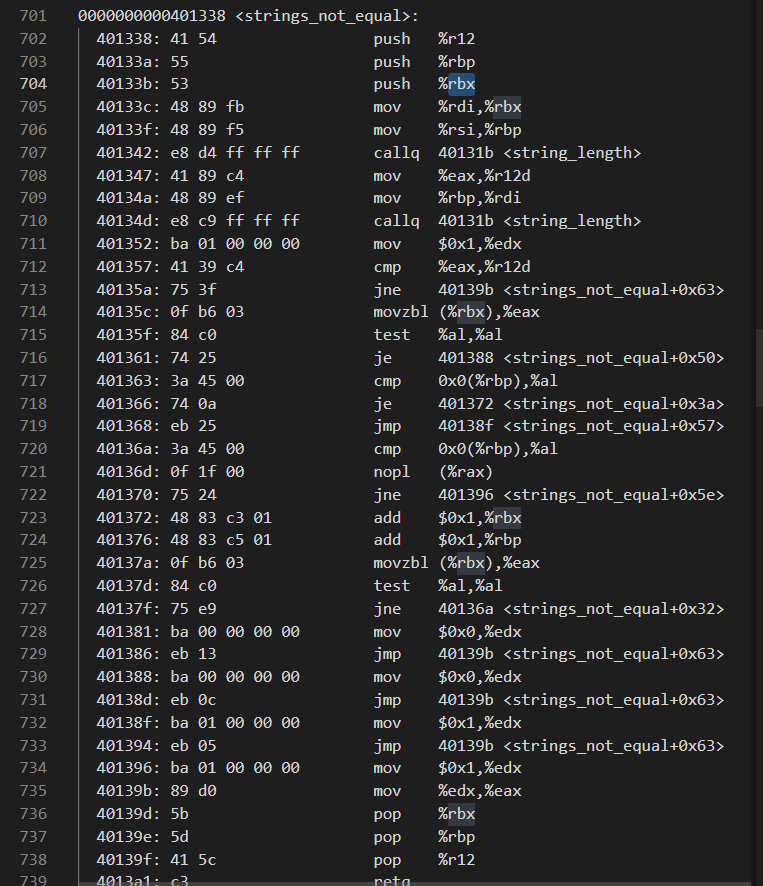
\includegraphics[scale=0.7]{image/2.2-2.png}
    \end{figure} 
    \item 第705,706行表明了传入参数有\%rdi和\%rsi,其中\%rsi的后32位存储了立即数0x402400。这两行将这两个参数存储到\%rbx和\%rbp这两个callee\-free寄存器中。
          接着调用了string\_length函数,猜测可能是求字符串长度的函数。
    \begin{figure}[htbp]
    % \centering
    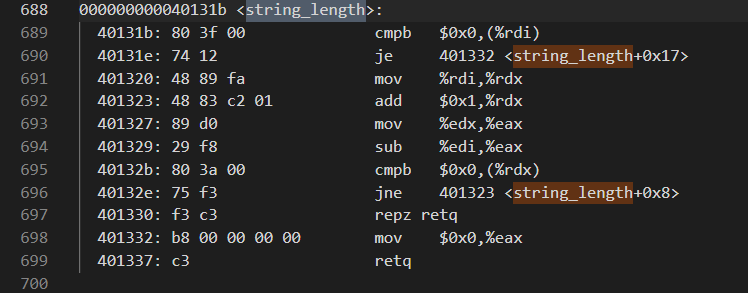
\includegraphics[scale=0.7]{image/2.2-3.png}
    \end{figure} 
    \item 观察string\_legnth函数,可知传入参数应该是字符串指针,该函数的大致作用是:
          将字符串指针一个一个往后指,同时更新字符串长度,如果指针指向了0x0,即字符串末尾的'\textbackslash0'则返回。
    \item 回过头来继续观察strings\_not\_equal函数,我们可以理解:到710行为止,函数求出了输入字符串的长度,存放在\%r12d中,
          答案字符串的长度,存放在\%eax中。接下来将\%edx赋值为1,判断两个字符串长度是否相等,如果不相等则跳转到735行,最后函数会返回1。
          接下来判断输入字符串中当前是否为空,为空则返回0,不为空则往后一个字符一个字符比较,一旦不相等就返回1。这基本验证了我们的猜想,所以本题的答案应该就是phase\_1函数中\%esi寄存器所存储的指针所指向的字符串。
    \item 所以我们只需要gdb 22300240028.out 并x/s 0x402400查看答案字符串即可。
    \begin{figure}[htbp]
    % \centering
    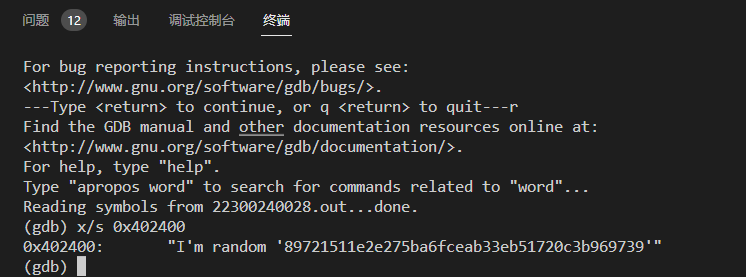
\includegraphics[scale=0.7]{image/2.2-4.png}
    \end{figure}
    \item phase\_1 defuse成功!
    \begin{figure}[htbp]
    % \centering
    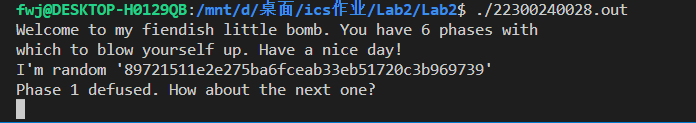
\includegraphics[scale=0.68]{image/2.2-5.png}
    \end{figure}
\end{itemize}

\subsection{phase\_2}
\begin{figure}[htbp]
% \centering
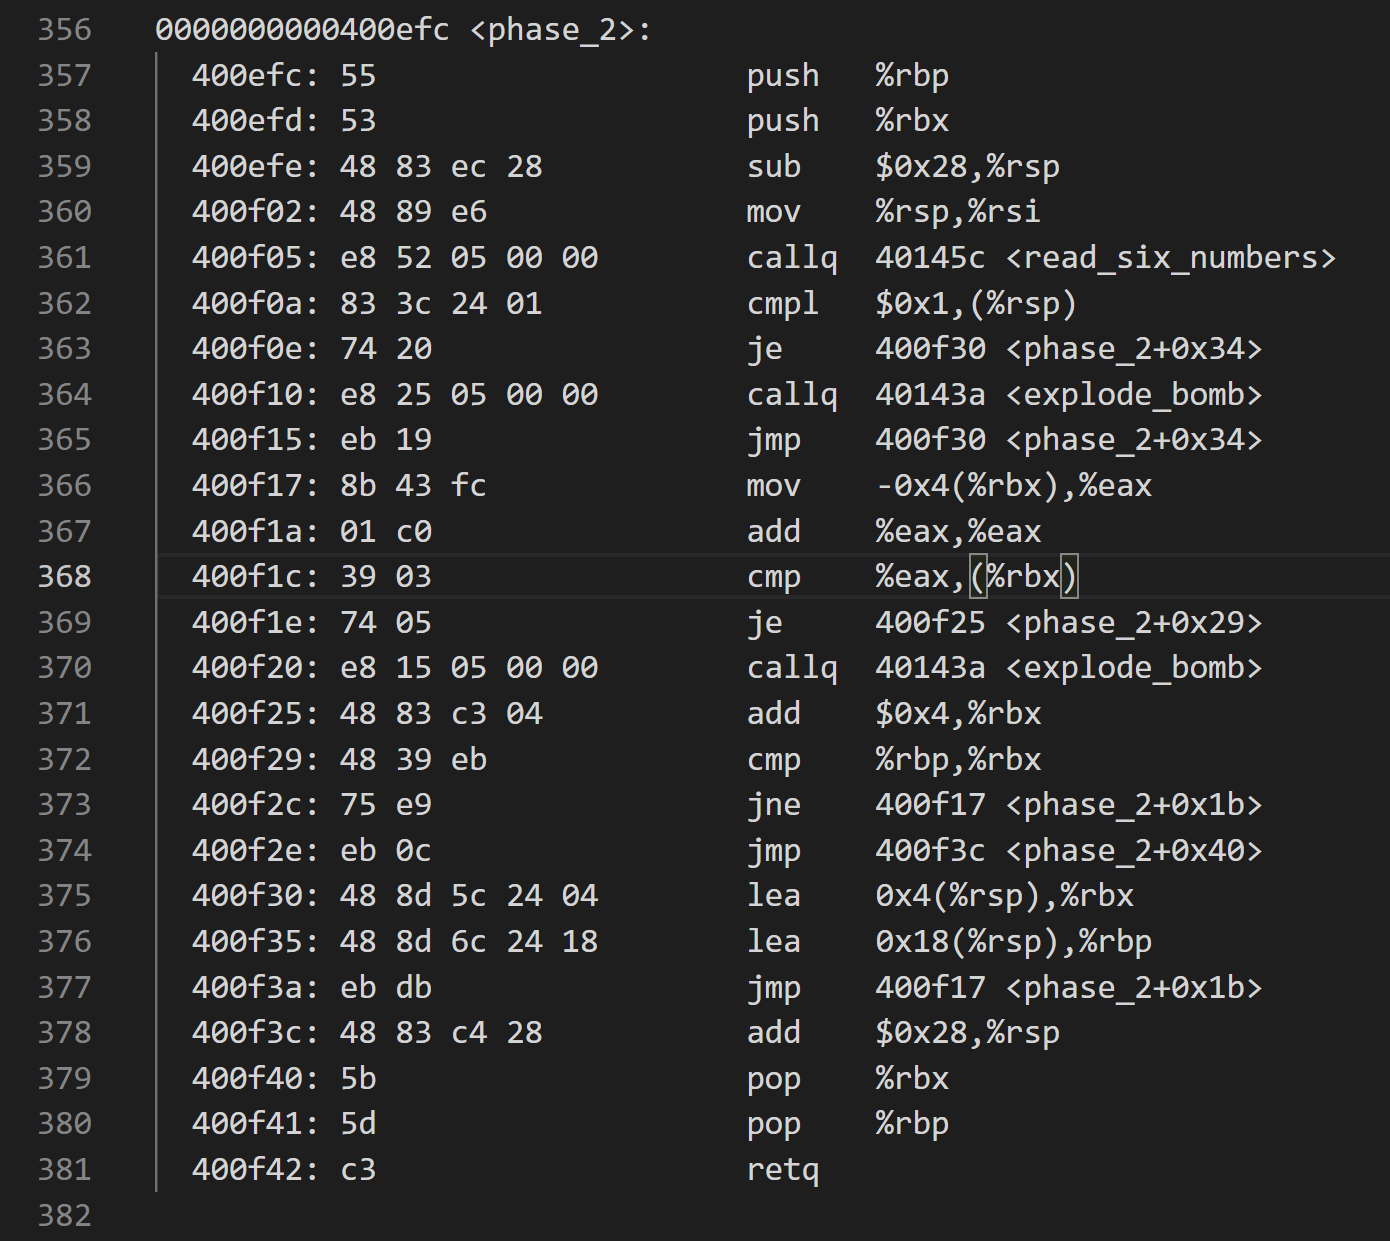
\includegraphics[scale=0.4]{image/2.3-1.png}
\end{figure}
\begin{itemize}
    \item 前四行压入寄存器,分配栈帧,保存\%rsp的值到\%rsi。接下来调用了函数read\_six\_numbers。
    \begin{figure}[htbp]
    % \centering
    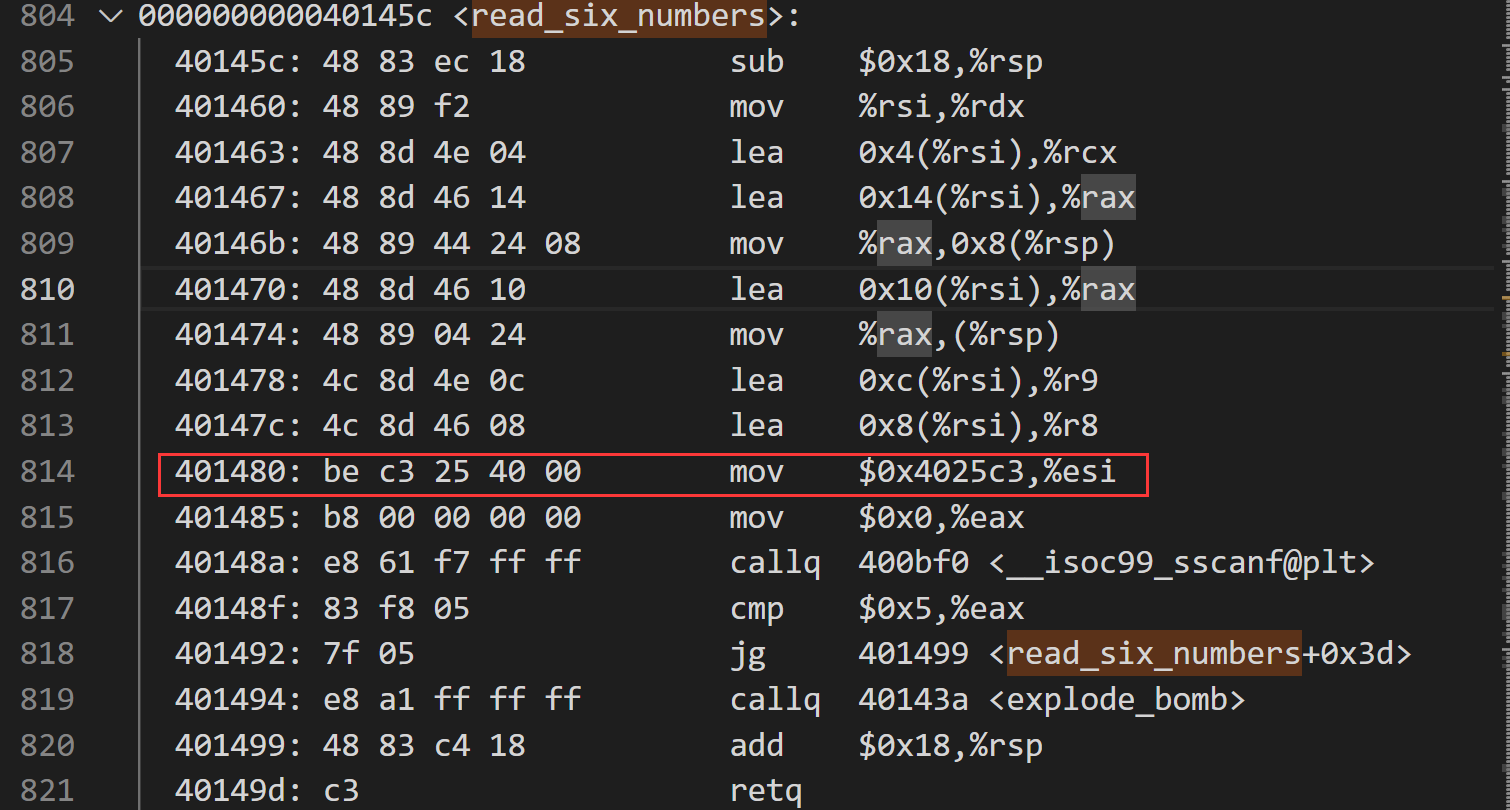
\includegraphics[scale=0.4]{image/2.3-2.png}
    \end{figure}  
    \item 在read\_six\_numbers函数中,我们发现805到813行运用lea和mov为寄存器赋值,而814行将一个看起来像地址一样的值赋给了\%esi,不妨用gdb查看一下。可以猜想我们需要输入六个整数并以空格隔开。
    \begin{figure}[htbp]
    % \centering
    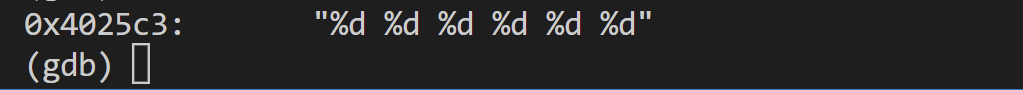
\includegraphics[scale=0.4]{image/2.3-3.png}
    \end{figure}   
    \item 再回过头来看phase\_2函数。读入后首先判断栈顶指针指向的地址的值,即$M[R[\%rsp]]$是否为1。
    接下来不难发现是一个循环:以\%rbx为计数器指针,每次加4,以\%rbp为终点指针,0x18 $/$ 0x4刚好等于6,
    意味着循环5次。在每次循环中\%eax存储之前的\%rbx寄存器指向的地址的值,并翻倍,与现在的寄存器\%rbx寄存器指向的地址的值进行比较,
    如果不一样就会使得炸弹爆炸。
    \item 因此可以大致得出答案是1 2 4 8 16 32。
    \item 不过这么判断的前提是:read\_six\_numbers函数会将$M[R[\%rsp]], M[R[\%rsp] + 0x4], \dots, M[R[\%rsp] + 0x14]$设置成输入的六个整数。
    因此我们还需要回过头来看一下这个函数一开始的寄存器赋值操作。
    \item \%rdi和\%rsi(原来的栈顶)作为前两个参数传入。read\_six\_numbers函数又将$M[R[\%rsi]], M[R[\%rsi] + 0x4], \cdots, M[R[\%rsi] + 0x14]$作为第3到8个传入参数,由于超出寄存器数量限制,最后两个参数被转移到内存上。
    如下图所示。同时我们可以看到这个函数的结尾处的跳出判定是大于5就可以,也就是说我们可以在答案结尾添加任意字符(和数字分开即可),例如:1 2 4 8 16 32*。
    \begin{figure}[htbp]
    % \centering
    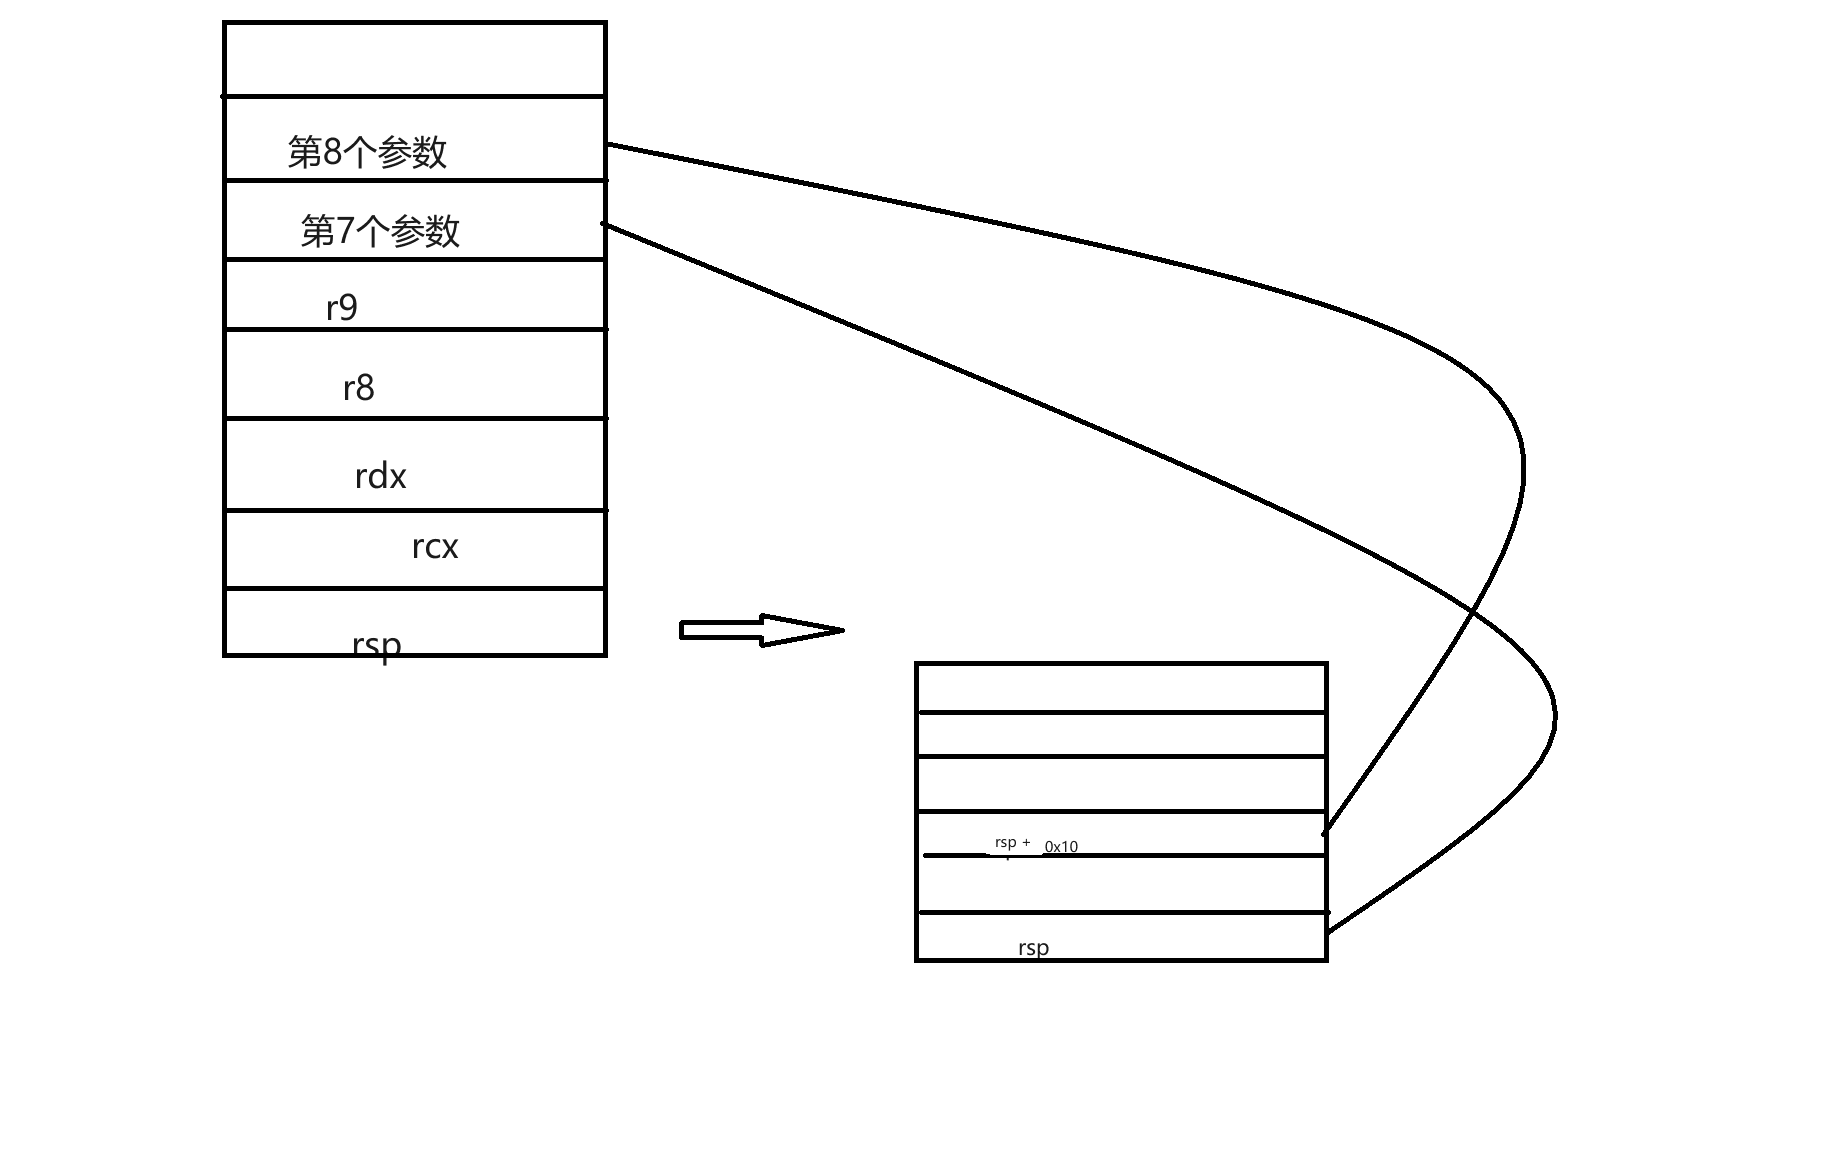
\includegraphics[scale=0.6]{image/2.3-4.png}
    \end{figure}  
    \item phase\_2 defuse成功!
    \begin{figure}[htbp]
    % \centering
    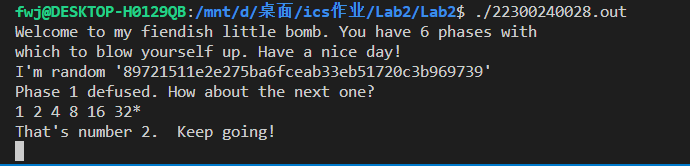
\includegraphics[scale=0.6]{image/2.3-5.png}
    \end{figure}       
\end{itemize}

\subsection{phase\_3}
\begin{figure}
    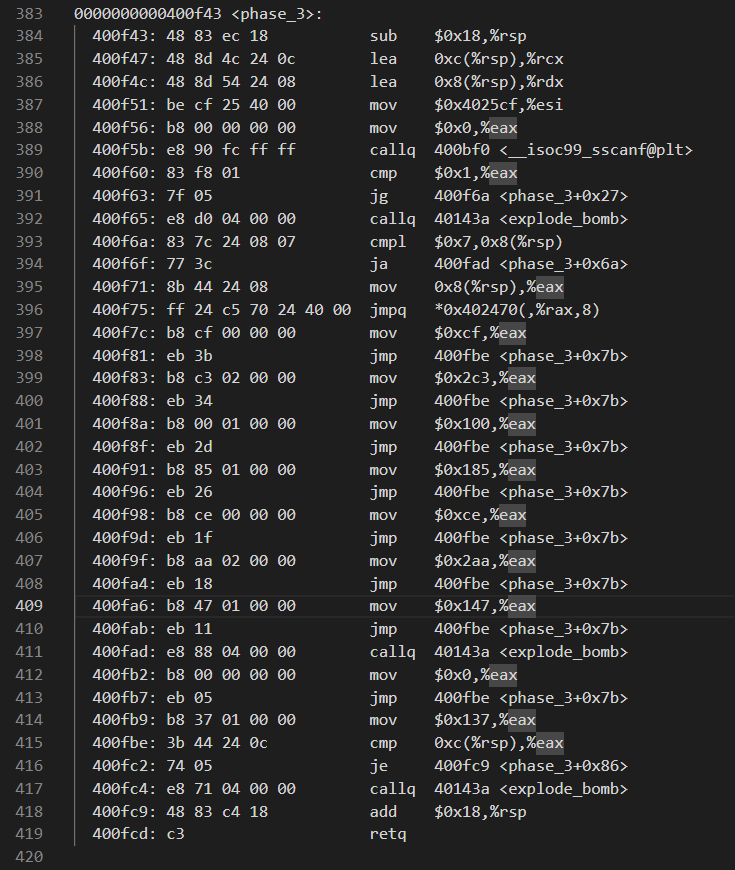
\includegraphics[scale=0.7]{image/2.4-1.png}
\end{figure}
\begin{itemize}
    \item 在第387行可以发现和phase\_2函数中类似的读入,用gdb调试后可知需要输入两个整数,以空格隔开。同样可以在答案结尾添加任意字符(和数字分开即可)。
    \begin{figure}[htbp]
        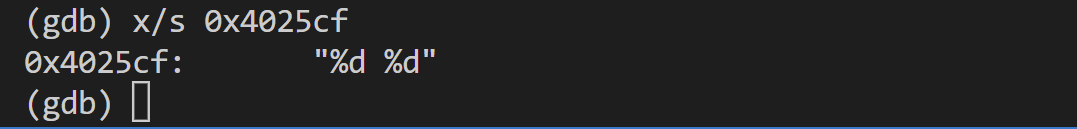
\includegraphics[scale=0.5]{image/2.4-2.png}
    \end{figure}
    \item 第393和394行表示如果$M[R[\%rsp] + 8] > 7$就会爆炸。接下来是一个奇怪的间接跳转,跳转到$M[0x402470 + 8 * R[\%rax]]$,注意这段地址储存在内存中。
    注意到之前将$M[R[\%rsp] + 8]$赋值给了\%eax,所以\%rax是一个小于等于7的无符号型整数。所以跳转到的地址有:\\$M[0x402470], M[0x402478], \cdots, M[0x4024a8]$这8种情况。
    不妨用gdb查看一下。发现这分别与第397,414,399,401,403,405,407,409行相对应。
    \begin{figure}[htbp]
        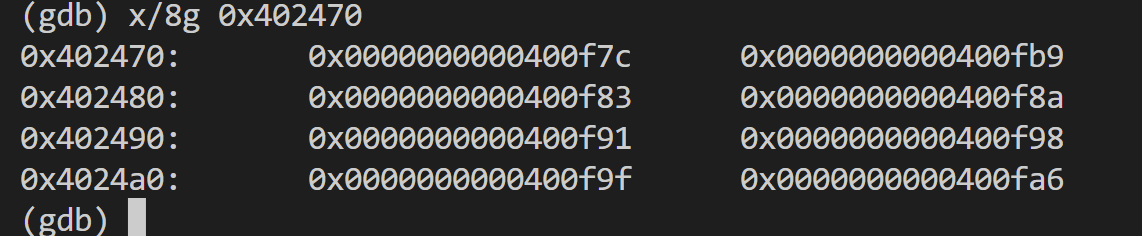
\includegraphics[scale=0.5]{image/2.4-3.png}
    \end{figure}
    \item 然后将\%eax赋值为一个常数,并跳转到第415行比较第二个参数和这个常数是否相等,不相等则爆炸。
    因此我们可以得出答案为:\\
    \\
\begin{tabular}{cc}
    \toprule
    第一个参数 & 第二个参数\\
    \midrule
    0 & 207\\
    1 & 311\\
    2 & 707\\
    3 & 256\\
    4 & 389\\
    5 & 206\\
    6 & 682\\
    7 & 327\\
    \bottomrule
\end{tabular}
    \item 我们取0 207*。phase\_3 defuse成功!
\begin{figure}[htbp]
    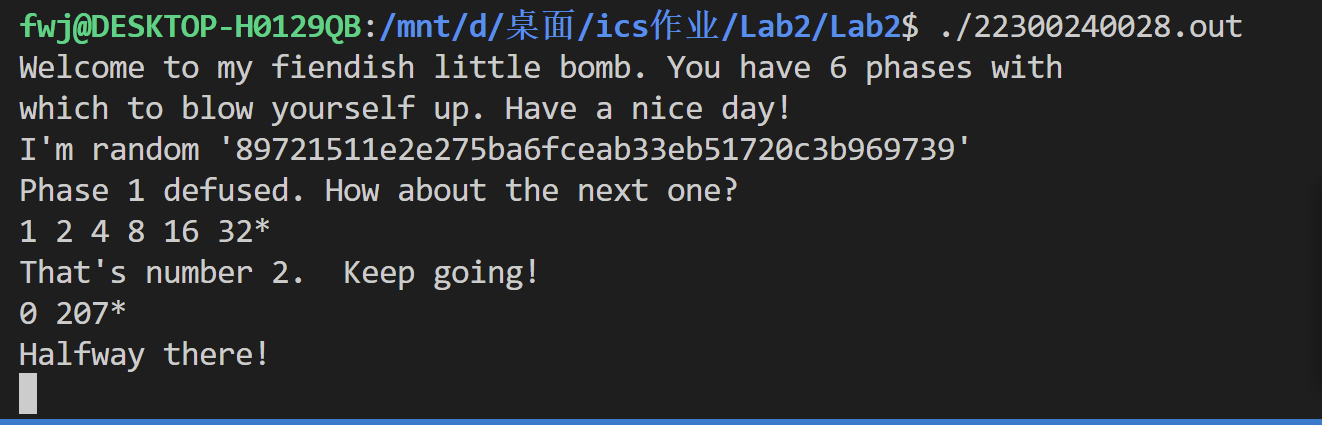
\includegraphics[scale=0.4]{image/2.4-4.png}
\end{figure}
\end{itemize}

\subsection{phase\_4}
\begin{figure}[htbp]
    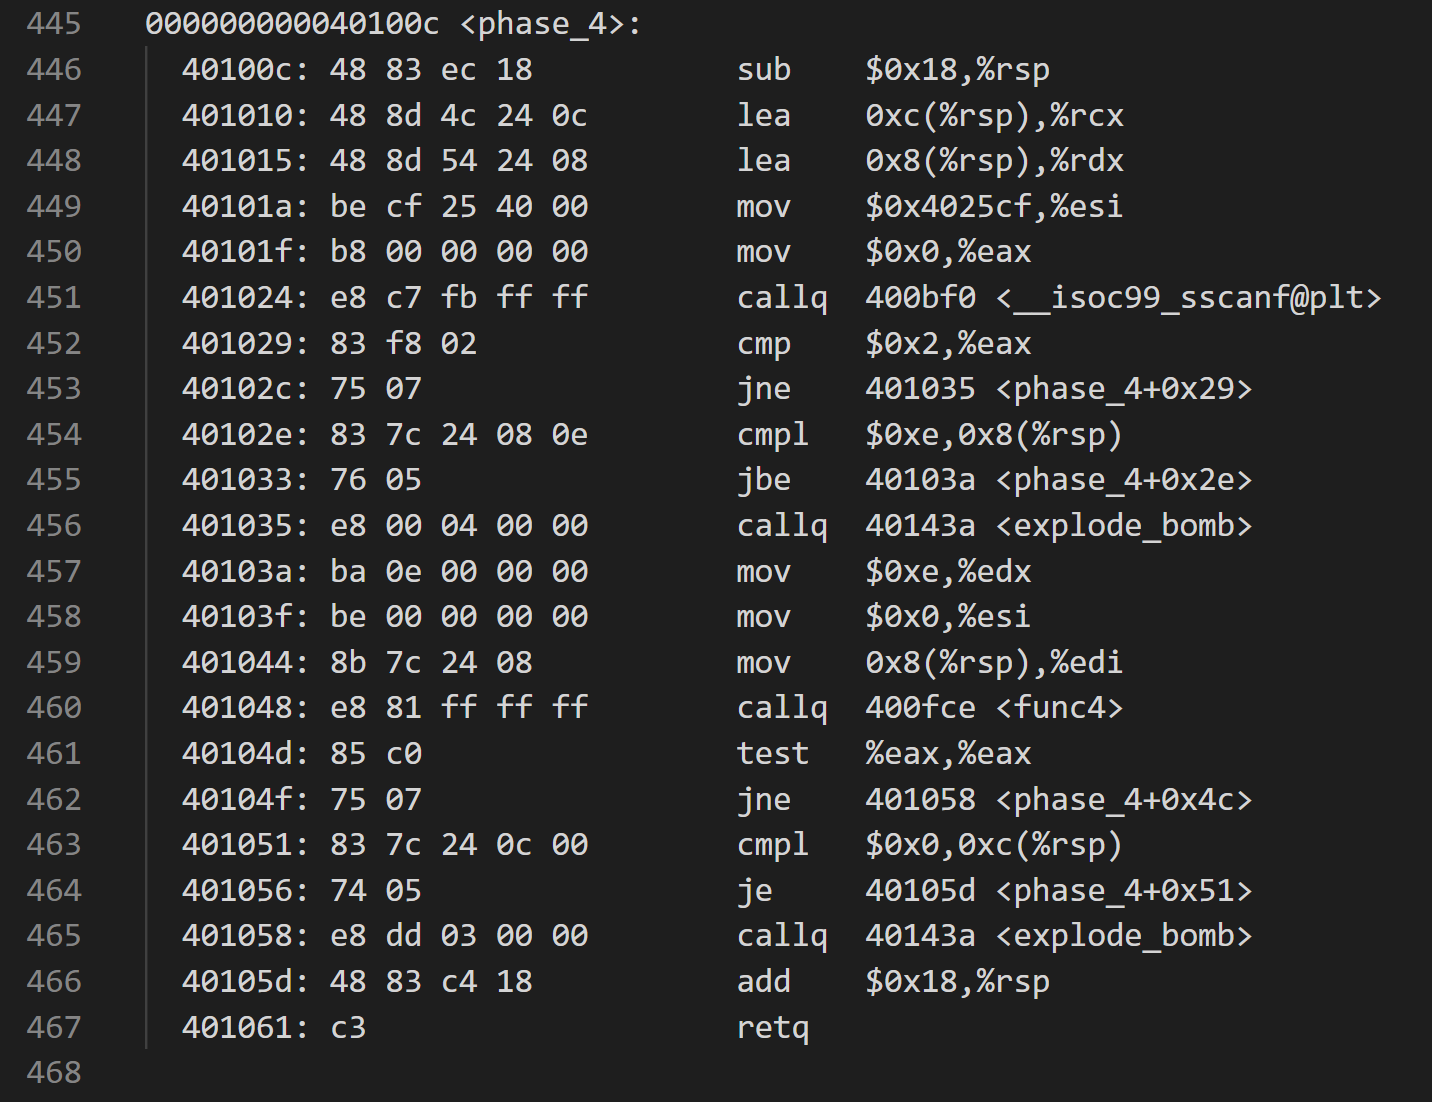
\includegraphics[scale=0.4]{image/2.5-1.png}
\end{figure}
\begin{itemize}
    \item 同phase\_3,在第449行经gdb调试(x/s 0x4025cf)可知需要输入两个整数。但是根据判断条件(第452,453行),\underline{我们需要输入三个参数}。
    \begin{figure}[htbp]
        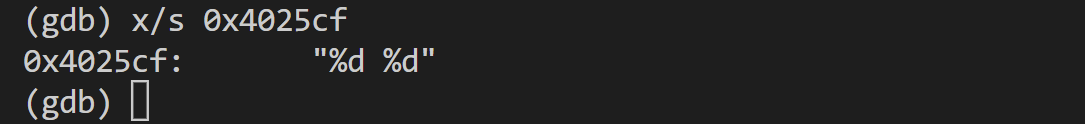
\includegraphics[scale=0.55]{image/2.5-2.png}
    \end{figure}    
    \item 首先判断输入的第一个整数是否小于等于0xe,如果大于则爆炸,小于则把\%edx赋成0xe、把\%esi赋成0x0、把$M[R[\%rsp] + 8]\le 0xe$赋给\%edi,调用fun\_4并传入参数。
    如果该函数返回值为0,并且第二个参数为0,则可以跳过爆炸。
    \begin{figure}[htbp]
        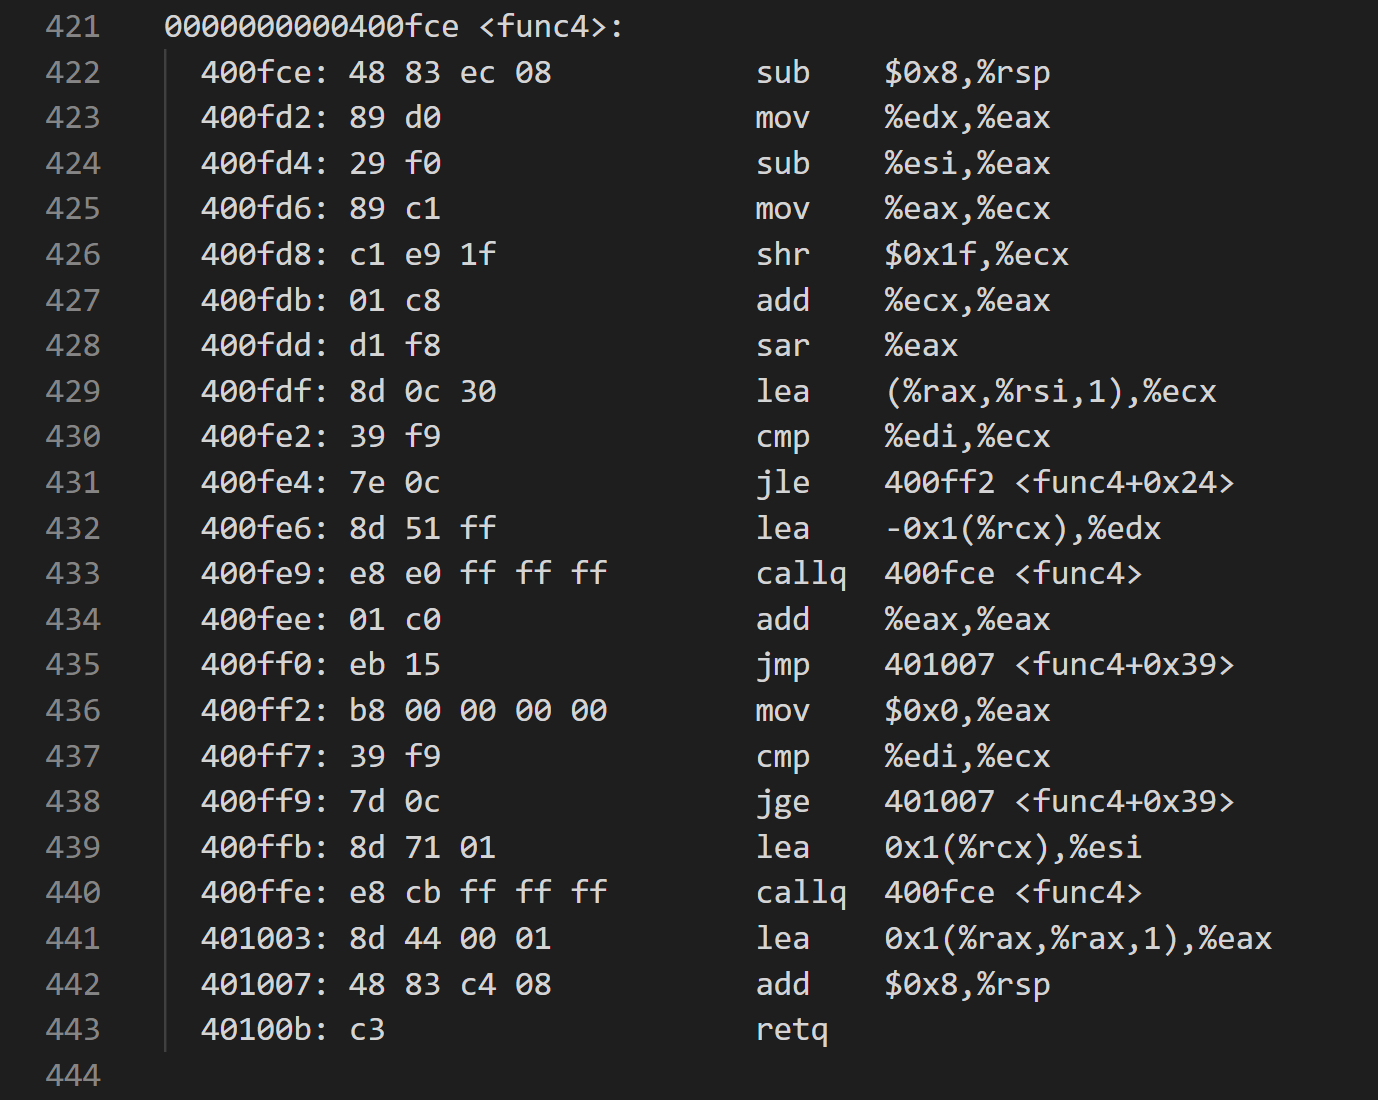
\includegraphics[scale=0.45]{image/2.5-3.png}
    \end{figure}  
    \item 可以看出该函数是一个递归函数,我们写出它对应的C语言代码来进行分析。为了直接求出答案,我们遍历所有可能的输入值。
\begin{lstlisting}
#include <stdio.h>
int cnt = 0;
int flag = 0; 
//edi=input, edx = 14, esi = 0
int fun_4(int esi, int edx, int edi)
{
    cnt ++;
    if(cnt >= 10000) {
        flag = 1;
        return 10086;
    }
    int eax = edx;
    eax -= esi;
    //eax = edx - esi;
    int ecx = eax;
    //ecx >>= 31;
    for(int i = 1; i <=31; i ++) ecx /= 2;
    eax += ecx;
    eax >>= 1;
    //eax = (eax + eax>>31)>>1;
    ecx = eax + esi;
    if(ecx > edi){
        edx = ecx - 1;
        return 2 * fun_4(esi, edx, edi);

    }else{
        eax = 0;
        if(ecx >= edi){
            return eax;
        }else{
            esi = ecx - 1;
            return 2 * fun_4(esi, edx, edi) + 1;
        }
    }
}
int main()
{
    for(int i = 0; i <= 14; i ++){
        cnt = 0;
        flag = 0;
        int res = fun_4(0, 14, i);
        if(!flag)
            printf("i=%d %d\n", i , res);
        else
            printf("i=%d No result\n", i);
    }
    return 0;
}
\end{lstlisting}
\begin{figure}[htbp]
    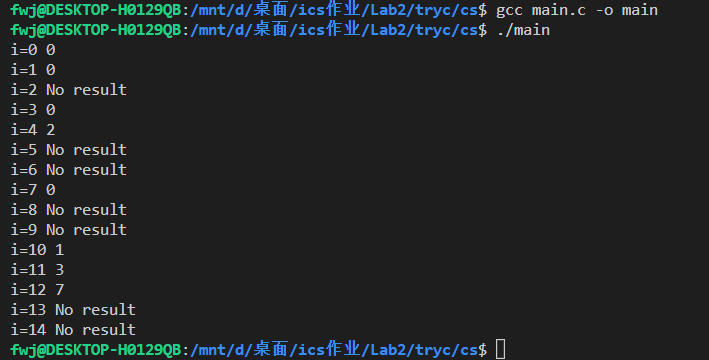
\includegraphics[scale=0.7]{image/2.5-4.png}
\end{figure}
    \item 这里的C程序假设了\%eax = \%rax,会导致有的输入进入死循环,不过这已经可以得出部分答案,足以跳过爆炸了。\\
    \\
    \begin{tabular}{cc}
        \toprule
        第一个参数 & 第二个参数\\
        \midrule
        0 & 0\\
        1 & 0\\
        3 & 0\\
        7 & 0\\
        \bottomrule
    \end{tabular}
    \item 我们取7 0。phase\_4 defuse成功!
    \begin{figure}[htbp]
        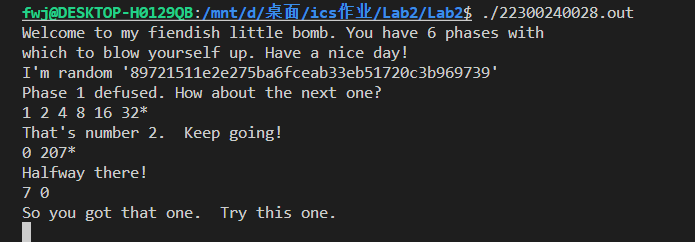
\includegraphics[scale=0.7]{image/2.5-5.png}
    \end{figure}
\end{itemize}

\subsection{phase\_5}
\begin{figure}[htbp]
    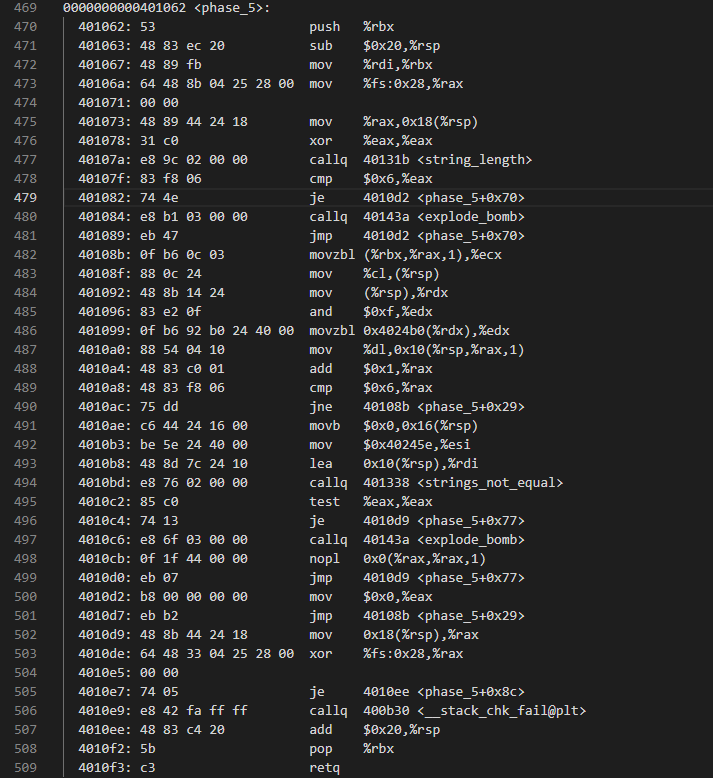
\includegraphics[scale=0.7]{image/2.6-1.png}
\end{figure}
\begin{itemize}
    \item 第477行调用string\_length函数求出输入字符串的长度,必须是6,否则爆炸。
    然后将\%rax从1到5循环:每次将$M[R[\%rbx] + R[\%rax]]$的后8位存在\%rdx中并只取它后四位(\&0xf)。
    把它作为索引找到$M[0x4024b0 + R[\%rdx]]$,取它的后8位存到$R[\%rsp] + R[\%rax] + 0x10$中。最后在结尾加上$'\backslash0'$.
    并和\%esi寄存器所存储的指针所指向的字符串相比较,如果相等则跳过爆炸。
    \item 用gdb调试得到0x4024b0和0x40245e处的字符串。
    \begin{figure}[htbp]
        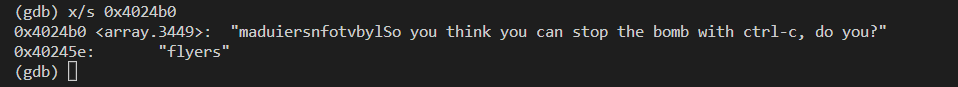
\includegraphics[scale=0.6]{image/2.6-2.png}
    \end{figure}    
    \item 我们需要在第一个字符串里找第二个字符串的字母。也就是说,我们输入的6个字符的后四位十进制值必须是9 15 14 5 6 7。
    \item 编写C语言程序可以快速得到我们要找的答案。
\begin{lstlisting}
#include <stdio.h>
int main()
{
    for(int i = 0; i <= 255; i ++)
    {
        if(i % 16 == 5)
            printf("5: %c\n", i);
        else if(i % 16 == 6)
            printf("6: %c\n", i);
        else if(i % 16 == 7)
            printf("7: %c\n", i);
        else if(i % 16 == 9)
            printf("9: %c\n", i);
        else if(i % 16 == 14)
            printf("e: %c\n", i);
        else if(i % 16 == 15)
            printf("f: %c\n", i);
    }
    return 0;
}    
\end{lstlisting}
\begin{figure}[htbp]
    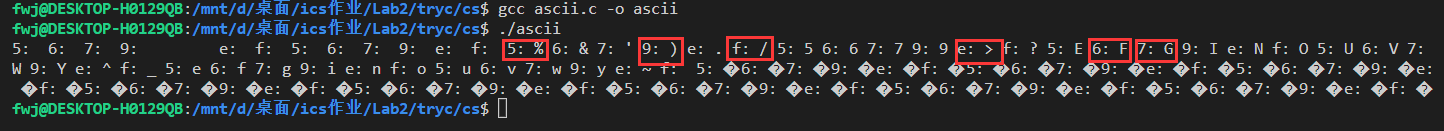
\includegraphics[scale=0.45]{image/2.6-3.png}
\end{figure}
    \item 不妨取$)/>\%FG$。phase\_5 defuse成功!
\begin{figure}[htbp]
    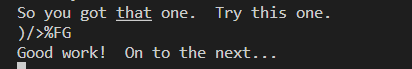
\includegraphics[scale=0.7]{image/2.6-4.png}
\end{figure}
\end{itemize}

\subsection{phase\_6}
\begin{figure}[htbp]
    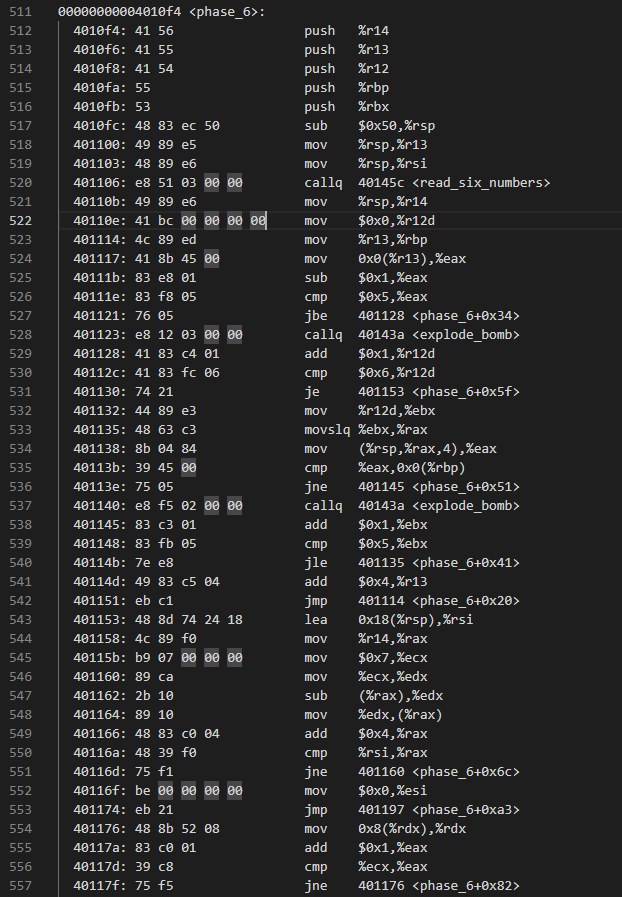
\includegraphics[scale=0.5]{image/2.7-1.png}
    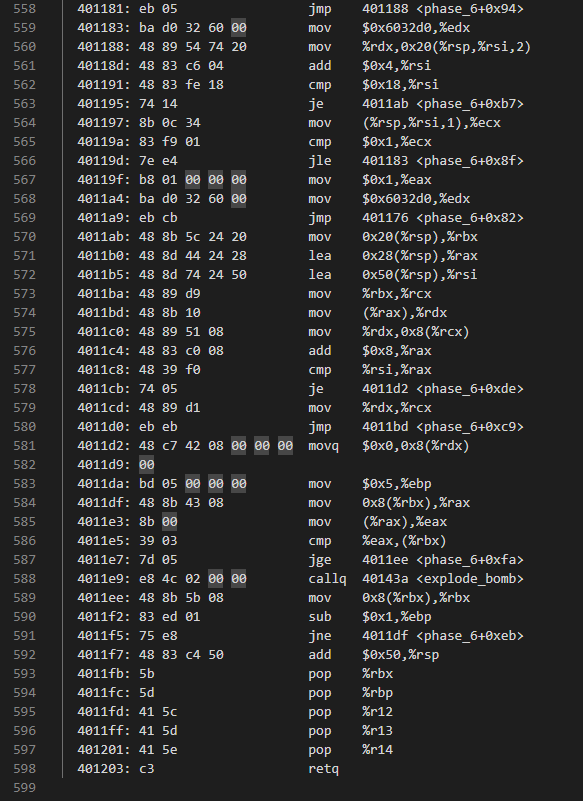
\includegraphics[scale=0.56]{image/2.7-2.png}
\end{figure}
\begin{itemize}
    \item 第520行看到read\_six\_numbers函数可知调用者的栈上按顺序存储了输入的六个数。接下来到542行为止是循环中套了循环,需要保证:每个数字小于等于6且互不相同。其C语言代码如下:
\begin{lstlisting}
r14 = 0;
r13 = 0;
r12d = 0;
while(1){           
    rbp = r13;
    if(num[r13] - 1 > 5)    
        goto bomb;
    r12d++;         
    if(r12d == 6)
        break;
    for(ebx = r12d; ebx <= 5; ebx++){   
        if(num[ebx] == num[rbp])       
            goto bomb;
    }
    r13++;
}    
\end{lstlisting}
    \item 接下来到551行是一个循环:将六个整数分别赋值成为用7减去它们自身。
    \item 接下来到569行是一个链表操作,通过我们输入的6个数字为索引对链表进行重排。
    即$M[R[\%rsp] + 0x20] = node[M[R[\%rsp]]], M[R[\%rsp] + 0x28] = node[M[R[\%rsp] + 0x4]], \cdots, M[R[\%rsp] + 0x48] = node[M[R[\%rsp] + 0x14]]$。 
    \begin{figure}[htbp]
        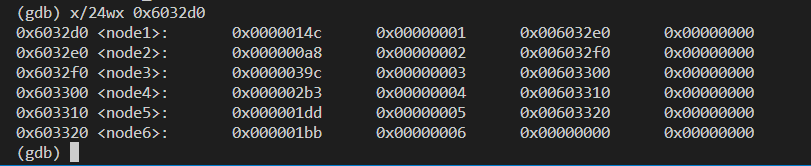
\includegraphics[scale=0.6]{image/2.7-3.png}
    \end{figure}
    \item 接下来到580行按照栈内链表节点位置顺序重排单链表。即原来链表的$1\to2\to\cdots\to6$顺序被修改为$M[R[\%rsp]] \to M[R[\%rsp]+0x4] \to\cdots\to M[R[\%rsp]+0x14]$
    \item 最后的循环是用来判断新链表是否是非严格单调递减的。由于:$node3>node4>node5>node6>node1>node2$,所以栈中的六个数应该是3 4 5 6 1 2。由于输入的数被7减过,所以答案应该是:4 3 2 1 6 5。
    \item phase\_6 defuse成功!
    \begin{figure}[htbp]
        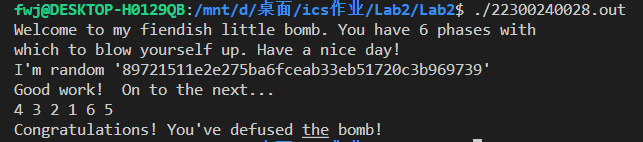
\includegraphics[scale=0.7]{image/2.7-4.png}
    \end{figure}
\end{itemize}

\subsection{secret\_phase}
\begin{itemize}
    \item 我们发现bomb.s中还有secret\_phase函数,但是之前没有遇到。Ctrl+F查询发现phase\_defused函数调用了它。用gdb查看一些地址的字符串时发现了隐藏关卡的突破口:
    当我们在某个关卡中要输入三个参数,并且最后一个参数是"HiEvil"时就能开启隐藏关卡。检查了一下前面的发现phase\_4需要我们输入三个参数,但是只有前两个参数在当时是有用的。
    \begin{figure}[htbp]
        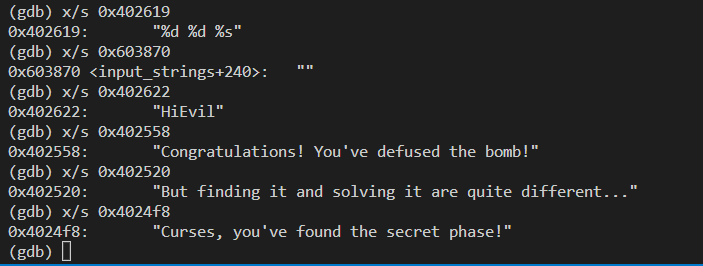
\includegraphics[scale=0.7]{image/2.8-1.png}
    \end{figure}
    \item 尝试了一下,开启了隐藏关卡。
    \begin{figure}[htbp]
        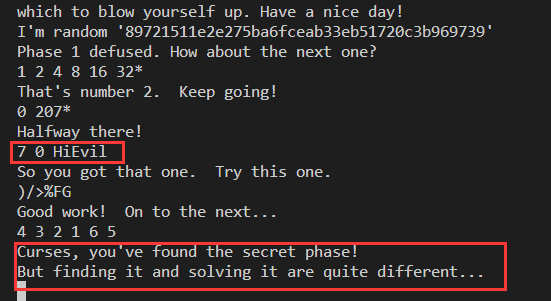
\includegraphics[scale=0.5]{image/2.8-2.png}
    \end{figure}
    \item 发现在secret\_phase中也有read\_line,说明我们要在最后再输入一个参数。这个参数和一个地址0x6030f0作为两个参数传入fun\_7函数,我们需要使得这个函数的返回值为2。
    \item 查看这个地址,发现是一个树型结构。
    \begin{figure}[htbp]
        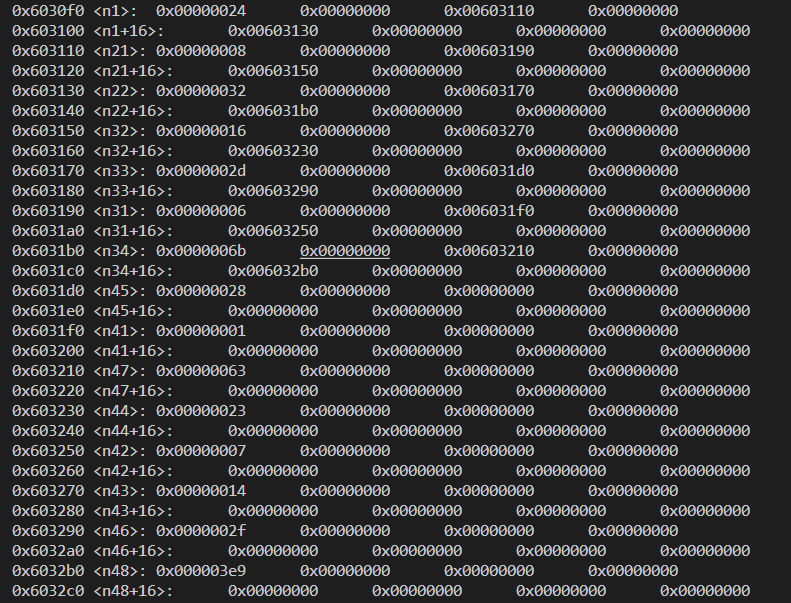
\includegraphics[scale=0.5]{image/2.8-3.png}
    \end{figure}    
    \item 画出示意图。
    \begin{figure}[htbp]
        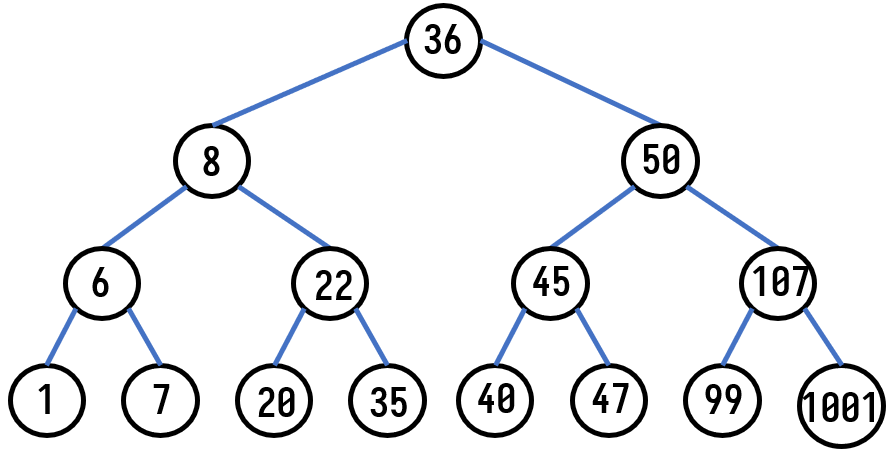
\includegraphics[scale=0.4]{image/2.8-4.png}
    \end{figure}     
    \item 查看fun\_7函数,发现是一个递归函数,写出其C语言代码。
\begin{lstlisting}
int fun7(Tree* rdi, int esi) {
    if (!rdi)   
        return -1;  
    if (rdi->val == esi)    
        return 0;       
    else if (rdi->val < esi)        
        return 2 * fun7(rdi -> right, esi) + 1;
    else
        return 2 * fun7(rdi -> left, esi);  
}    
\end{lstlisting}
    \item 要使得其返回2,需要先从左子树返回1。要想返回1,需要先从右子树返回0。所以我们从36开始,esi一定小于36;进入左子树,esi一定大于8;进入右子树esi一定等于22。故答案为22。
    \item secret\_phase defuse成功!
\end{itemize}

\subsection{答案ans.txt}
\noindent
I'm random '89721511e2e275ba6fceab33eb51720c3b969739'\\
1 2 4 8 16 32*\\
0 207*\\
7 0 HiEvil\\
$)/>\%FG$ \\
4 3 2 1 6 5\\
20\\
22300240028\\
\end{document}

